\documentclass{beamer}
%
% Choose how your presentation looks.
%
% For more themes, color themes and font themes, see:
% http://deic.uab.es/~iblanes/beamer_gallery/index_by_theme.html
%
\mode<presentation>
{
  \usetheme{default}      % or try Darmstadt, Madrid, Warsaw, ...
  \usecolortheme{default} % or try albatross, beaver, crane, ...
  \usefonttheme{default}  % or try serif, structurebold, ...
  \setbeamertemplate{navigation symbols}{}
  \setbeamertemplate{caption}[numbered]
  \setbeamertemplate{footline}[frame number]
} 

\usepackage[english]{babel}
\usepackage[utf8x]{inputenc}
\usepackage{listings}
\usepackage{courier}
\usepackage{array}
\usepackage{dirtree}

\title[2016-05-11-scala-spark]{Scala and Spark Tutorial}
\author{Jim Pivarski}
\institute{Princeton University -- DIANA}
\date{May 11, 2016}

\xdefinecolor{darkblue}{rgb}{0.1,0.1,0.7}
\xdefinecolor{darkgrey}{rgb}{0.35,0.35,0.35}
\definecolor{commentgreen}{rgb}{0,0.6,0}
\definecolor{stringmauve}{rgb}{0.58,0,0.82}

\lstset{ %
  backgroundcolor=\color{white},      % choose the background color
  basicstyle=\ttfamily\scriptsize,         % size of fonts used for the code
  breaklines=true,                    % automatic line breaking only at whitespace
  captionpos=b,                       % sets the caption-position to bottom
  commentstyle=\color{commentgreen},  % comment style
  escapeinside={\%*}{*)},             % if you want to add LaTeX within your code
  keywordstyle=\color{blue},          % keyword style
  stringstyle=\color{stringmauve},    % string literal style
  showstringspaces=false,
  showlines=true
}

\lstdefinelanguage{scala}{
  morekeywords={abstract,case,catch,class,def,%
    do,else,extends,false,final,finally,%
    for,if,implicit,import,match,mixin,%
    new,null,object,override,package,%
    private,protected,requires,return,sealed,%
    super,this,throw,trait,true,try,%
    type,val,var,while,with,yield},
  otherkeywords={=>,<-,<\%,<:,>:,\#,@},
  sensitive=true,
  morecomment=[l]{//},
  morecomment=[n]{/*}{*/},
  morestring=[b]",
  morestring=[b]',
  morestring=[b]"""
}

\begin{document}

\begin{frame}
  \titlepage
\end{frame}

% Uncomment these lines for an automatically generated outline.
%\begin{frame}{Outline}
%  \tableofcontents
%\end{frame}

\begin{frame}{}
\begin{description}
\item[Spark:] a data analysis framework

{\small (like ROOT, but with different strengths and weaknesses).}

\vspace{0.5 cm}

\item[Scala:] Spark's native language, used as a command prompt

{\small (the way that C++ is used in ROOT).}
\end{description}
\end{frame}

\begin{frame}{Outline}
\begin{enumerate}
\item 5 minute talk on Scala
\item $\sim$half hour Scala exercises
\item 5 minute talk on Spark
\item $\sim$hour and a half Spark exercises in Scala
\item 10 minute intro to Histogrammar
\end{enumerate}
\end{frame}

\begin{frame}{}
\begin{columns}
\column{1.1\linewidth}
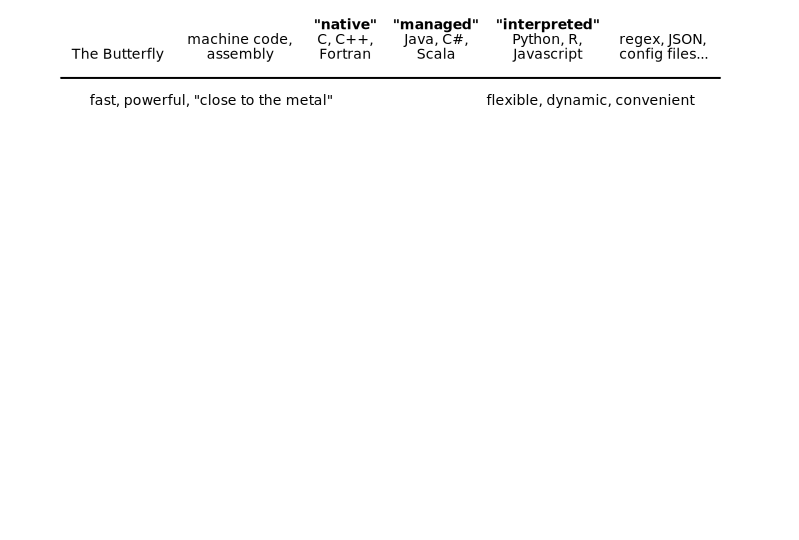
\includegraphics[width=\linewidth]{languages1.pdf}
\end{columns}
\end{frame}

\begin{frame}{}
\begin{columns}
\column{1.1\linewidth}
\includegraphics[width=\linewidth]{languages2.pdf}
\end{columns}
\end{frame}

\begin{frame}{}
\begin{columns}
\column{1.1\linewidth}
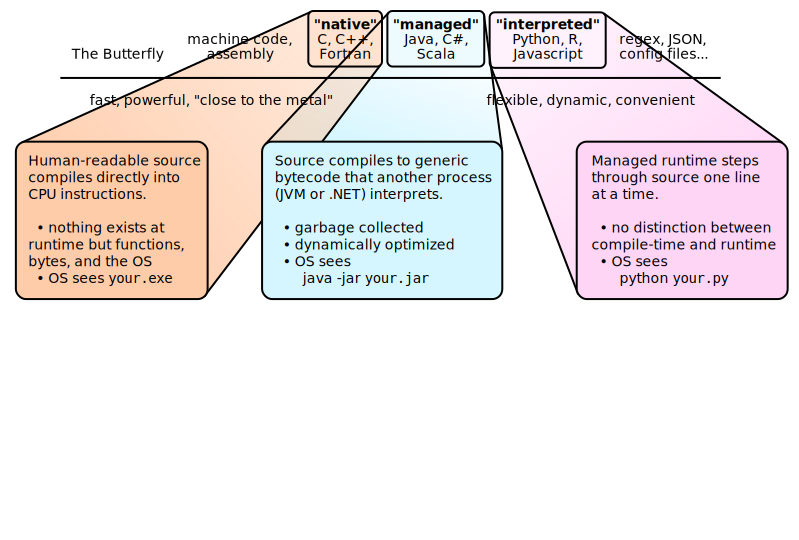
\includegraphics[width=\linewidth]{languages25.pdf}
\end{columns}
\end{frame}

\begin{frame}{}
\begin{center}
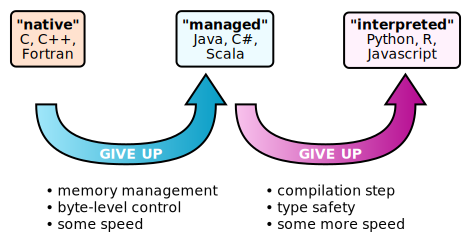
\includegraphics[width=0.8\linewidth]{languages3.pdf}
\end{center}
\end{frame}

\begin{frame}{}
\begin{center}
\includegraphics[width=0.8\linewidth]{languages4.pdf}
\end{center}
\end{frame}

\begin{frame}{What happens in the compilation step?}
\begin{itemize}
\item Whole program is interpreted and turned into machine instructions (possibly for a virtual machine).
\item All variables are interpreted as belonging to specific types: {\tt \small int}, {\tt \small string}, {\tt \small MissileController}\ldots
\item Uses of these variables are checked for validity:
\begin{itemize}
\item can't pass a {\tt \small MissileController} into the cosine function;
\item can't call {\tt \small launchAllMissiles()} on a {\tt \small string}.
\end{itemize}
\end{itemize}

\vfill
Interpreted languages do none of these things; you find out about misuses of variables at runtime (can be good, can be bad).
\end{frame}

\begin{frame}{Why should you care?}
\begin{itemize}
\item Compilation step can get in the way of testing a program one piece at a time.
\item The type check is a {\it formal proof} that the program is free of certain types of errors; it won't fail after hours of running.
\end{itemize}

\vfill
\begin{uncoverenv}<2->
\hspace{-0.83 cm} \textcolor{darkblue}{\Large Scala}

\begin{itemize}
\item Scala compiles to bytecode that runs on the Java Virtual Machine (JVM).
\item It emphasizes type safety (even more than C++).
\item It has extensive type inference to reduce annoyance,
\item and an interactive prompt for testing small components or interacting with a running program.
\end{itemize}
\end{uncoverenv}
\end{frame}

\begin{frame}{}
\begin{columns}
\column{1.18\linewidth}
\includegraphics[width=\linewidth]{jvm_languages.png}
\end{columns}
\end{frame}

\begin{frame}{}
\begin{columns}
\column{1.18\linewidth}
\includegraphics[width=\linewidth]{popularity1.png}
\end{columns}
\end{frame}

\begin{frame}{}
\begin{columns}
\column{1.18\linewidth}
\includegraphics[width=\linewidth]{popularity2.png}
\end{columns}
\end{frame}

\begin{frame}{}
\begin{center}
\Huge \textcolor{darkblue}{Scala Exercises}
\end{center}
\end{frame}

{\usebackgroundtemplate{\includegraphics[width=\paperwidth]{word-cloud-07-2014_full.png}}
\begin{frame}{Big Data tools}
\end{frame}
}

{\usebackgroundtemplate{\includegraphics[width=\paperwidth]{word-cloud-07-2014.png}}
\begin{frame}{Big Data tools}
\begin{columns}
\column{0.4\linewidth}

\textcolor{darkblue}{Batch data analysis:}

\begin{itemize}
\item Apache Hadoop
\item {\only<1>{Apache Spark}\only<2>{\bf \textcolor{red}{Apache Spark}}}
\item Google TensorFlow
\end{itemize}

\textcolor{darkblue}{Query engines:}

\begin{itemize}
\item Elasticsearch
\item Apache Impala
\item Apache Drill
\item {\only<1>{Spark-SQL}\only<2>{\bf \textcolor{red}{Spark-SQL}}}
\end{itemize}

\textcolor{darkblue}{Data pipelines:}

\begin{itemize}
\item Apache Kafka
\item nsq
\end{itemize}

\column{0.4\linewidth}
\textcolor{darkblue}{Streaming data analysis:}

\begin{itemize}
\item Apache Storm
\item Apache Flink
\item {\only<1>{Spark-Streaming}\only<2>{\bf \textcolor{red}{Spark-Streaming}}}
\end{itemize}

\textcolor{darkblue}{Cluster infrastructures:}

\begin{itemize}
\item Apache HDFS
\item Apache Mesos
\end{itemize}

\textcolor{darkblue}{Machine learning:}

\begin{itemize}
\item Scikit-Learn
\item Apache Mahout
\item {\only<1>{Spark MLlib}\only<2>{\bf \textcolor{red}{Spark MLlib}}}
\end{itemize}
\end{columns}

\hfill \textcolor{blue}{\scriptsize \url{https://github.com/onurakpolat/awesome-bigdata}}
\end{frame}}

\begin{frame}{From Hadoop to Spark}
\vspace{-0.1 cm}
\begin{block}{2003--2004}
Google published {\it The Google File System} and {\it MapReduce: Simplified Data Processing on Large Clusters.}
\end{block}

\begin{block}{2006}
HDFS and Hadoop-MapReduce projects started at \\ Yahoo!\ but within Apache, fully open-source.

\vspace{-1.4 cm} \hfill \includegraphics[width=2 cm]{01_Hadoop_full.jpg}
\end{block}

\begin{block}{2008--2009}
Hadoop sorted TB--PB of data in record time. Started getting contributions from Facebook, LinkedIn, eBay, and IBM.
\end{block}

\begin{block}{2009}
Spark began as a class project at Berkley, targeting \\ {\it iterative} map-reduce for machine learning.

\vspace{-1.1 cm} \hfill \includegraphics[width=2 cm]{spark-logo.png}
\end{block}

\begin{block}{2013}
Spark became an Apache project and Databricks founded. In 2014, Spark won records for TB--PB sorting.
\end{block}
\end{frame}

\begin{frame}{Google Trends search results}
\begin{center}
\includegraphics[width=0.9\linewidth]{trends.png}
\end{center}
\end{frame}

\begin{frame}{}
\begin{columns}
\column{0.65\linewidth}
\textcolor{darkblue}{Spark's specialty:} caching data in RAM for iterative fits.

\vspace{0.2 cm}
Hadoop (and every other distributed batch system I've heard of) has to load data from disk for each pass.

\column{0.35\linewidth}
\includegraphics[width=\linewidth]{spark_time.png}
\end{columns}

\vfill
Beyond this killer app, Spark was designed for exploratory data analysis; Hadoop was designed for large applications.
\begin{itemize}
\item Native Spark runs on a command line in Scala (natively), Python, and R (through a bridge).
\item Hadoop asks the user to extend Mapper and Reducer classes.
\item Spark has many minor conveniences.
\item Spark generalizes on the map-reduce concept to chains of functional primitives.
\end{itemize}
\end{frame}

\begin{frame}[fragile]{Chains of functional primitives}

Functional programming style is common among data analysts using R (inherited from Scheme).

\vspace{0.2 cm}
\uncover<2->{Scala's object orientation lets us chain functors without nesting.}

\vspace{0.2 cm}
\begin{columns}
\column{0.6\linewidth}
\begin{lstlisting}[language=c,frame=single]
for (i = 0;  i < nEvents;  i++) {
    event = events(i);
    if (condition(event))
        continue;
    add_to_output(calculation(event));
}
\end{lstlisting}
\column{0.42\linewidth}
\begin{onlyenv}<1>
\begin{lstlisting}[language=python,frame=single]

output = 
  map(calculation,
    filter(condition,
                events))

\end{lstlisting}
\end{onlyenv}
\begin{onlyenv}<2->
\begin{lstlisting}[language=python,frame=single]

output =
  events.filter(condition)
        .map(calculation)


\end{lstlisting}
\end{onlyenv}
\end{columns}

\begin{uncoverenv}<3->
\begin{itemize}
\item The ``map'' functor {\it says less} than ``for''--- it doesn't specify an order in which events must be processed.
\item Underlying system can distribute and collect however it likes.
\item Also hides index arithmetic from the user: datasets can be spliced automatically.
\end{itemize}
\end{uncoverenv}
\end{frame}

\begin{frame}{``Monad-like'' functional primitives:}

Transforming one data table (ntuple) into another.

\vfill
\renewcommand{\arraystretch}{1.5}
\begin{tabular}{p{0.12\linewidth} >{\centering}p{0.08\linewidth} >{\centering}p{0.17\linewidth} >{\centering}p{0.08\linewidth} p{0.4\linewidth}}
& input & function & output & operation \\\hline
\textcolor{darkblue}{map} & table of $A$ & $f: A \to B$ & table of $B$ & apply $f$ to each row $A$, get a table of the same number of rows $B$ \\
& \multicolumn{4}{l}{\scriptsize \color{darkgrey} a.k.a. ``lapply'' (R), ``SELECT'' (SQL), list comprehension (Python)} \\
\textcolor{darkblue}{filter} & table of $A$ & $f: A \to \mbox{boolean}$ & table of $A$ & get a shorter table with the same type of rows \\
& \multicolumn{4}{l}{\scriptsize \color{darkgrey} a.k.a. single brackets (R), ``WHERE'' (SQL), list comprehension (Python)} \\
\textcolor{darkblue}{flatMap} & table of $A$ & $f: A \to \mbox{table of } B$ & table of $B$ & compose \textcolor{darkblue}{map} and \textcolor{darkblue}{flatten}, get a table of any length \\
& \multicolumn{4}{l}{\scriptsize \color{darkgrey} a.k.a. ``map'' (Hadoop), ``EXPLODE'' (SQL), $>>=$ (Haskell)} \\
\end{tabular}
\end{frame}

\begin{frame}{``Monoid-like'' functional primitives:}

Summarizing an ntuple using a counter, summation, or histogram.

\vfill
\renewcommand{\arraystretch}{1.5}
\begin{tabular}{p{0.12\linewidth} >{\centering}p{0.2\linewidth} >{\centering}p{0.23\linewidth} >{\centering}p{0.08\linewidth} >{\raggedright\arraybackslash}p{0.25\linewidth}}
& input & function(s) & output & operation \\\hline
\textcolor{darkblue}{reduce} & table of $A$ & $f: (A, A) \to A$ & single $A$ & apply $f$ to the running sum and one more element \\
\textcolor{darkblue}{aggregate} & table of $A$, initial value $B$ (``zero'') & $f: (A, B) \to B$ $f: (B, B) \to B$ (increment and combine) & single value $B$ & accumulate a counter with a different data type from the input \\
\textcolor{darkblue}{aggregate by key} & table of $\langle K,A \rangle$, initial value $B$ & $f: (A, B) \to B$ $f: (B, B) \to B$ & pairs $\langle K,B \rangle$ & aggregate independently for each key \\
& \multicolumn{4}{l}{\scriptsize \color{darkgrey} a.k.a. ``reduce'' (Hadoop), ``GROUP BY'' (SQL)} \\
\end{tabular}
\end{frame}

\begin{frame}{Associativity is key}

``Monad'' and ``monoid'' refer to mathematical properties of the operator, the most important being associativity, which allows the user's function to be dispatched arbitrarily.

\begin{center}
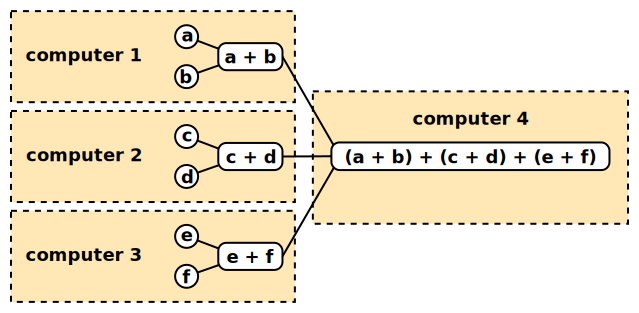
\includegraphics[width=0.7\linewidth]{monoids.pdf}
\end{center}
\end{frame}

\begin{frame}{}
\begin{center}
\Huge \textcolor{darkblue}{Spark Exercises}
\end{center}
\end{frame}

\begin{frame}[fragile]{Histogrammar}
We want to avoid downloading the whole dataset to a laptop for a traditional ntuple-analysis.

\vspace{0.5 cm}
Spark has a functional for reducing data in a distributed way:

\begin{center}
\tt \small RDD.aggregate(initialize)(increment, combine)
\end{center}

where
\begin{itemize}
\item {\tt \small RDD} is a collection of data of type $\mathcal{D}$ (end of skimming chain)
\item {\tt \small initialize} creates a counter of type $\mathcal{C}$
\item {\tt \small increment} is a function from $(\mathcal{C},\mathcal{D}) \to \mathcal{C}$
\item {\tt \small combine} is a function from $(\mathcal{C},\mathcal{C}) \to \mathcal{C}$
\end{itemize}
\end{frame}

\begin{frame}{Aggregate functional}

\begin{center}
\tt \small RDD.aggregate(initialize)(increment, combine)
\end{center}

\vfill
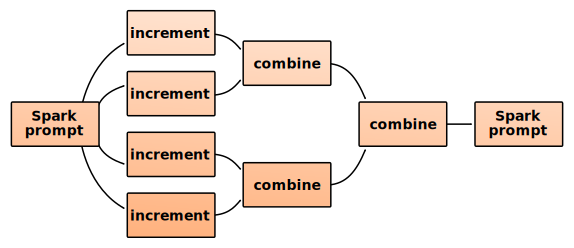
\includegraphics[width=\linewidth]{aggregate.pdf}

\vfill
(Hadoop equivalent: reduce; \hspace{0.25 cm} SQL equivalent: ``{\tt GROUP BY}'')
\end{frame}

\begin{frame}[fragile]{Histograms fit naturally into aggregate}

\begin{lstlisting}[language=scala]
// hypothetical import ROOT
import org.dianahep.scaroot.classes.TH1F

val finalHist = RDD.aggregate(
    // "booking"
    new TH1F("pt", "pt", 100, 0, 20))(
    // "filling"
    {(h, d) => h.Fill(sqrt(d.px**2 + d.py**2)); h},
    // "merging"
    {(h1, h2) => h1.Add(h2); h1})
\end{lstlisting}

\uncover<2>{\begin{block}{}
\vspace{-\baselineskip}
Not bad, but what if you want to fill more than one histogram?

\begin{itemize}
\item These are {\it functions:} all histograms must be passed in as arguments and collected as return values ({\tt \small h} and {\tt \small h1} above).
\item No global state because Spark is distributed.
\item Data analyst has to maintain histogram code in three places.
\end{itemize}
\end{block}}
\end{frame}

\begin{frame}[fragile]{First idea:}
\textcolor{darkblue}{\large Move the logic of histogram-filling into the booking stage.}

\begin{lstlisting}[language=scala]
val h = Histogram("pt", 100, 0, 20,
                  {d => sqrt(d.px**2 + d.py**2)})
\end{lstlisting}

\vspace{-\baselineskip} \hfill $\underbrace{\mbox{\hspace{6.0 cm}}}_{\mbox{``fill rule'' } {\displaystyle f: \mathcal{D} \to \mathbb{R}}}$ \hspace{0.7 cm}

\vfill
This functional design allows the filling and merging to be automatic: no user input required.

\begin{lstlisting}[language=scala]
RDD.aggregate(h)(auto_increment(), auto_combine())
\end{lstlisting}
\end{frame}

\begin{frame}[fragile]{Second idea:}
\textcolor{darkblue}{\large Collect histograms into a container that also has automated filling and merging.}

\begin{lstlisting}[language=scala]
val pack_o_histograms = Label(
      "pt" -> Histogram(100, 0, 20, fill_pt),
      "Emiss" -> Histogram(100, 0, 50, fill_Emiss),
      ...)

RDD.aggregate(pack_o_histograms)(auto_increment(),
                                 auto_combine())
\end{lstlisting}

\vfill
({\tt \small Label} and {\tt \small Histogram} share a superclass; {\tt \small auto\_increment()} and {\tt \small auto\_combine()} call them the same way.)
\end{frame}

\begin{frame}[fragile]{Third idea:}
\vspace{0.5 cm}
\textcolor{darkblue}{\large Let all of these pieces be composable.}

\begin{lstlisting}[language=scala]
val directories =
      Label("dir1" ->
                Label("pt" -> Histogram(...),
                      "Emiss" -> Histogram(...)),
            "dir2" ->
                Label("pass" -> Count(...),
                      "maxpt" -> Maximize(...)))
\end{lstlisting}

\vspace{1.5 cm}
(Combining directories of histograms is similar to ROOT's {\tt \small hadd}.)
\end{frame}

\begin{frame}[fragile]{}
\textcolor{darkblue}{\large Notice that histograms themselves can be decomposed into smaller pieces:}

\begin{lstlisting}[language=scala]
val histogram = Histogram(100, 0, 20, fill_rule)
val histogram = Bin(100, 0, 20, fill_rule, Count())
\end{lstlisting}

where
\begin{itemize}
\item {\tt \small Count} is an aggregator that counts events;
\item {\tt \small Bin} is an aggregator that makes 100 sub-aggregators and uses {\tt \small fill\_rule} to decide which one to pass the data on to, just as {\tt \small Label} passes the data on to all of its contents.
\end{itemize}

\vspace{0.5 cm}
\begin{uncoverenv}<2->
We get two-dimensional histograms for free:
\begin{lstlisting}[language=scala]
val hist2d = Bin(binsX, lowX, highX, fillX,
                   Bin(binsY, lowY, highY, fillY, Count()))
\end{lstlisting}
\end{uncoverenv}
\vspace{-1.5 cm}
\end{frame}

\begin{frame}[fragile]{}
\vspace{0.5 cm}
With the right sub-aggregators, we can get profile plots:
\begin{lstlisting}[language=scala]
val profile = Bin(binsX, lowX, highX, fillX,
                                  Deviate(fillY))
  // "Deviate" accumulates mean & std deviation
\end{lstlisting}

Box-and-whisker plots:
\begin{lstlisting}[language=scala]
val box_whiskers = Bin(binsX, lowX, highX, fillX,
                         Branch(Quantile(fillY),
                                Minimize(fillY),
                                Maximize(fillY)))
  // "Quantile" accumulates median & quartiles
  // "Branch" makes a tree of subaggregators
\end{lstlisting}

Heatmaps (average per bin, not a two-dimensional histogram):
\begin{lstlisting}[language=scala]
val heatmap = Bin(binsX, lowX, highX, fillX,
                    Bin(binsY, lowY, fillY,
                          Average()))
  // "Average" accumulates a mean only
\end{lstlisting}
\end{frame}

\begin{frame}[fragile]{}
\textcolor{darkblue}{\large Mix and match with alternate binning schemes:}

\vspace{0.5 cm}
Fill a hashmap instead of an array:
\begin{lstlisting}[language=scala]
val unknown_support =
      SparselyBin(binWidth, fillX, Count())
  // "SparselyBin" creates subaggregators as needed
\end{lstlisting}

Non-uniform bins:
\begin{lstlisting}[language=scala]
val partitions_like_clustering =
      CentrallyBin(binCenters, fillX, Count())
val completely_arbitrary_bins =
      IrregularlyBin(binRanges, fillX, Count())
\end{lstlisting}

Use a clustering algorithm to find bin centers:
\begin{lstlisting}[language=scala]
val first_look = AdaptivelyBin(fillX, Count())

val violin_plot = Bin(binsX, lowX, highX, fillX,
                      AdaptivelyBin(fillY, Count())
\end{lstlisting}
\end{frame}

\begin{frame}[fragile]{}
\textcolor{darkblue}{\large Similarly for super-histogram structures:}

\vspace{0.5 cm}
\begin{lstlisting}[language=scala]
val efficiency = Fraction(cut, Histogram(...))
\end{lstlisting}
where {\tt \small cut} is a function from $\mathcal{D} \to$ bool; two identical histograms are booked, one (denominator) is filled with all events, the other (numerator) only if it passes the cut.

\vfill
\begin{lstlisting}[language=scala]
val stack = Stack(q, cuts, Histogram(...))
\end{lstlisting}
where {\tt \small q} is a function from $\mathcal{D} \to \mathbb{R}$ and {\tt \small cuts} are successively tighter thresholds; $N_{\mbox{\scriptsize cuts}} + 1$ histograms are created.

\vfill
\begin{lstlisting}[language=scala]
val partition = Partition(q, cuts, Histogram(...))
\end{lstlisting}
Histograms now represent data {\it between} cuts (think of centrality bins in heavy ion plots).
\end{frame}

\begin{frame}[fragile]{}
\textcolor{darkblue}{\large Categorical features, too:}

\vfill
Fill rule maps from $\mathcal{D} \to$ string:
\begin{lstlisting}[language=scala]
val bar_chart = Categorize(fillType, Count())
\end{lstlisting}
Order of categories on the axis can be imposed {\it after} aggregation. The data are accumulated in a hashmap.

\vfill
\begin{lstlisting}[language=scala]
val backgrounds =
     Categorize({d => d.eventType},
       Histogram(120, 0, 120, {d => d.dimuonMass}))
\end{lstlisting}

Stacking order can also be imposed {\it after} aggregation.
\end{frame}

\begin{frame}{}
\textcolor{darkblue}{\large A whole analysis can be a tree of nested histogram primitives with lambda functions at each level.}

\vfill
\dirtree{%
.1 {\tt \small Label}.
.2 {\tt \small "trigger thresholds"}.
.3 {\tt \small Stack} $\to$ {\tt \small Fraction} $\to$ {\tt \small Bin} $\to$ {\tt \small Count}.
.2 {\tt \small "cut scan"}.
.3 {\tt \small Stack} $\to$ {\tt \small Label}.
.4 {\tt \small "a vs b"} $\to$ {\tt \small Bin} $\to$ {\tt \small Deviate}.
.4 {\tt \small "b vs c"} $\to$ {\tt \small Bin} $\to$ {\tt \small Deviate}.
.2 {\tt \small "pT windows"}.
.3 {\tt \small Partition} $\to$ {\tt \small Label}.
.4 {\tt \small "a"} $\to$ {\tt \small Bin} $\to$ {\tt \small Count}.
.4 {\tt \small "b"} $\to$ {\tt \small Bin} $\to$ {\tt \small Count}.
}

\vfill
Can answer questions like, ``which cuts were applied in this plot?'' by walking the tree, rather than scanning a {\tt \small for} loop for {\tt \small break} statements by eye.
\end{frame}

\begin{frame}{Implementation}
I started implementing this grammar to see if it makes sense.

\begin{center}
\textcolor{blue}{\url{http://github.com/diana-hep/histogrammar/}}
\end{center}

(with an ``a,'' get it?)
\end{frame}

\begin{frame}{}
\vfill
\begin{minipage}{\linewidth}
\renewcommand{\arraystretch}{1.2}
\begin{tabular}{l c c c | l c c}
Primitive & Scala & Python & C++ & Primitive & Scala & Python \\\hline
{\bf \scriptsize Count}       & $\surd$ & $\surd$ & $\surd$ & {\bf \scriptsize CentrallyBin}    & $\surd$ & $\surd$ \\
{\bf \scriptsize Sum}         & $\surd$ & $\surd$ &      & {\bf \scriptsize AdaptivelyBin}   & $\surd$ & $\surd$ \\
{\bf \scriptsize Average}     & $\surd$ & $\surd$ &      & {\bf \scriptsize Fraction}        & $\surd$ & $\surd$ \\    
{\bf \scriptsize Deviate}     & $\surd$ & $\surd$ &      & {\bf \scriptsize Stack}           & $\surd$ & $\surd$ \\
{\bf \scriptsize AbsoluteErr} & $\surd$ & $\surd$ &      & {\bf \scriptsize Partition}       & $\surd$ & $\surd$ \\
{\bf \scriptsize Minimize}    & $\surd$ & $\surd$ &      & {\bf \scriptsize Categorize}      & $\surd$ & $\surd$ \\
{\bf \scriptsize Maximize}    & $\surd$ & $\surd$ &      & {\bf \scriptsize Limit}           & $\surd$ & $\surd$ \\
{\bf \scriptsize Quantile}    & $\surd$ & $\surd$ &      & {\bf \scriptsize Label}           & $\surd$ & $\surd$ \\
{\bf \scriptsize Bag}         & $\surd$ & $\surd$ &      & {\bf \scriptsize UntypedLabel}    & $\surd$ & $\surd$ \\
{\bf \scriptsize Bin}         & $\surd$ & $\surd$ & $\surd$ & {\bf \scriptsize Index}           & $\surd$ & $\surd$ \\
{\bf \scriptsize SparselyBin} & $\surd$ & $\surd$ &      & {\bf \scriptsize Branch}          & $\surd$ & $\surd$ \\
\end{tabular}
\end{minipage}

\vspace{0.5 cm}
Shared JSON representation so primitives can be freely exchanged.

\vfill
CUDA is next, along with hooks to popular plotting frameworks.
\end{frame}

\begin{frame}[fragile]{Example Spark session}
\begin{lstlisting}[language=scala]
import org.dianahep.histogrammar._
import org.dianahep.histogrammar.histogram._

// declare histograms
val px_histogram = Histogram(100, -5, 5,
  {mu: Muon => mu.px})
val pt_histogram = Histogram(80, 0, 8,
  {mu: Muon => sqrt(mu.px**2 + mu.py**2)})
val cut_histogram = Histogram(100, -5, 5,
  {mu: Muon => mu.px}, {mu: Muon => mu.py < 0})

// wrap them up in a collection
val all_histograms = Label("px" -> px_histogram,
  "pt" -> pt_histogram, "cut" -> cut_histogram)

// fill them in Spark
val final_result = rdd.aggregate(all_histograms)
      (new Increment, new Combine)
\end{lstlisting}
\end{frame}

\begin{frame}[fragile]{Example Spark session}
\begin{lstlisting}[language=scala]
all_histograms("pt").entries     // 0
final_result("pt").entries       // 100000
\end{lstlisting}

\begin{uncoverenv}<2->
\begin{lstlisting}[language=scala]
println(final_result("pt").ascii)
\end{lstlisting}
\tiny
\begin{verbatim}
                        0                                                   6616.50
                        +---------------------------------------------------------+
underflow          0    |                                                         |
[  0    ,  0.100)  506  |****                                                     |
[  0.100,  0.200)  1420 |************                                             |
[  0.200,  0.300)  2424 |*********************                                    |
[  0.300,  0.400)  3356 |*****************************                            |
[  0.400,  0.5  )  4258 |*************************************                    |
[  0.5  ,  0.600)  4688 |****************************************                 |
[  0.600,  0.700)  5262 |*********************************************            |
[  0.700,  0.800)  5805 |**************************************************       |
[  0.800,  0.900)  5855 |**************************************************       |
[  0.900,  1    )  6015 |****************************************************     |
[  1    ,  1.10 )  5977 |***************************************************      |
[  1.10 ,  1.20 )  5940 |***************************************************      |
[  1.20 ,  1.30 )  5763 |**************************************************       |
[  1.30 ,  1.40 )  5463 |***********************************************          |
[  1.40 ,  1.5  )  5009 |*******************************************              |
[  1.5  ,  1.60 )  4676 |****************************************                 |
[  1.60 ,  1.70 )  4226 |************************************                     |
[  1.70 ,  1.80 )  3743 |********************************                         |
[  1.80 ,  1.90 )  3226 |****************************                             |
[  1.90 ,  2    )  2911 |*************************                                |
[  2    ,  2.10 )  2449 |*********************                                    |
...
\end{verbatim}
\end{uncoverenv}
\end{frame}

\begin{frame}[fragile]{In Python\ldots}
\begin{lstlisting}[language=python]
th1f = final_result("pt").TH1F("name", "title")
th1f.Draw()
# because "import ROOT" didn't raise an ImportError
\end{lstlisting}

\includegraphics[width=\linewidth]{root_th1f.png}
\end{frame}

\begin{frame}{Histogrammar does not produce graphics}
\textcolor{darkblue}{\large (The ASCII art histogram is a placeholder/debugging/fun.)}

\vfill
Although any combination of the primitives can be aggregated and used in an analysis, special combinations like {\tt Bin(Count)} are recognized as plottable.

\vfill
Histogrammar should link to external packages, such as Matplotlib and ROOT, to do the actual plotting.
\begin{itemize}
\item Minimal codebase to reimplement in a variety of languages;
\item More of a clearinghouse than a software product, connecting systems that iterate over data to systems that plot data.
\end{itemize}
\end{frame}

\begin{frame}
\vspace{0.3 cm}
\hspace{-0.5 cm}\begin{minipage}{\linewidth}
\tiny
\renewcommand{\arraystretch}{1.3}
\begin{tabular}{| p{0.1\linewidth} p{0.9\linewidth} |}\hline
Count           & Count data, ignoring their content. (Actually a sum of weights.) \\\hline
Sum             & Accumulate the sum of a given quantity. \\
Average         & Accumulate the weighted mean of a given quantity. \\
Deviate         & Accumulate a weighted variance, mean, and total weight of a given quantity (using an algorithm that is stable for large numbers). \\
AbsoluteErr     & Accumulate the weighted Mean Absolute Error (MAE) of a quantity whose nominal value is zero. \\
Minimize        & Find the minimum value of a given quantity. If no data are observed, the result is NaN. \\
Maximize        & Find the maximum value of a given quantity. If no data are observed, the result is NaN. \\
Quantile        & Accumulate an adaptively binned histogram to compute approximate quantiles, such as the median. \\\hline
Bag             & Accumulate raw data up to an optional limit, at which point only the total number is preserved. \\\hline
Bin             & Split a given quantity into equally spaced bins between specified limits and fill only one bin per datum. \\
SparselyBin     & Split a quantity into equally spaced bins, filling only one bin per datum and creating new bins as necessary. \\
CentrallyBin    & Split a quantity into bins defined by a set of bin centers, filling only one datum per bin with no overflows or underflows. \\
AdaptivelyBin   & Split a quanity into bins dynamically with a clustering algorithm, filling only one datum per bin with no overflows or underflows. \\\hline
Fraction        & Accumulate two containers, one with all data (denominator), and one with data that pass a given selection (numerator). \\
Stack           & Accumulate a suite containers, filling all that are above a given cut on a given expression. \\
Partition       & Accumulate a suite containers, filling the one that is between a pair of given cuts on a given expression. \\
Categorize      & Split a given quantity by its categorical (string-based) value and fill only one category per datum. \\\hline
Label           & Accumulate any number of containers of the SAME type and label them with strings. Every one is filled with every input datum. \\
UntypedLabel    & Accumulate containers of any type except Count and label them with strings. Every one is filled with every input datum. \\
Index           & Accumulate any number of containers of the SAME type anonymously in a list. Every one is filled with every input datum. \\
Branch          & Accumulate containers of DIFFERENT types, indexed by i0 through i9. Every one is filled with every input datum. \\\hline
\end{tabular}
\end{minipage}
\end{frame}

\end{document}
